% V2 working paper: compact ICAPS-style presentation of the Playbook model.
\documentclass[letterpaper]{article}
\usepackage[draft]{aaai2026}
\usepackage{times}
\usepackage{helvet}
\usepackage{courier}
\usepackage[hyphens]{url}
\usepackage{graphicx}
\urlstyle{rm}
\def\UrlFont{\rm}
\usepackage{natbib}
\usepackage{caption}
\frenchspacing
\setlength{\pdfpagewidth}{8.5in}
\setlength{\pdfpageheight}{11in}

\usepackage{amsthm}

\theoremstyle{definition}
\newtheorem{definition}{Definition}

\usepackage{amsmath,amssymb}
\usepackage{algorithm}
\usepackage{algorithmic}
\usepackage{newfloat}
\usepackage{listings}
\usepackage{tikz}
\usetikzlibrary{arrows.meta,positioning,calc}

\DeclareCaptionStyle{ruled}{labelfont=normalfont,labelsep=colon,strut=off}
\lstset{
  basicstyle=\footnotesize\ttfamily,
  numbers=none,
  aboveskip=3pt,
  belowskip=3pt,
  showstringspaces=false,
  tabsize=2,
  breaklines=true
}
\floatstyle{ruled}
\newfloat{listing}{tb}{lst}{}
\floatname{listing}{Listing}

\pdfinfo{
/TemplateVersion (2026.1)
}
\setcounter{secnumdepth}{1}

\title{Finite Agent Machines}
\author{Dustin Dannenhauer}
\affiliations{
  Delegance AI\\
  \texttt{dustin@delegance.ai}
}

\begin{document}
\maketitle

% ---------------------------------------------------------------------------
% Fresh draft: replace each TBD as you rewrite the paper.
% ---------------------------------------------------------------------------
\begin{abstract}
TBD
\end{abstract}

\section{Introduction}

Conclusively verifying software outcomes is fundamentally unsolveable for most software. This is evidenced by the sheer number of techniques used to incrementally assure software is correct including unit tests, in-code assertions, human review, compiler and type checking, static analysis and linters, fuzzing, ... etc. Conclusive verification is the bottleneck that prevents brute forcing solutions or otherwise. Large Langage Models are improving the ability to search the space of software solutions for improvements in algorithms and software more generally. We say that a solution is \textit{conclusively verifiable} if the checker gaurauntees that incorrect outcomes are never accepted (soundness), correct outcomes are not rejected (completeness), and the checker always returns an answer for every candidate (totality). For problems where you have a conclusive verifier, the cost of solving that problem boils down to the cost running the verifier and the cost of searching the space of solutions for problems worth checking. If the gains of finding a solution is greater than the estimated cost to search and the cost to verify, then it is worth it to do the search. 

In this paper we propose a novel solution to perform solution search when there is no conclusive verifier with cheap cost. Our solution is a novel multi-agent policy with  human-oversight. 





 the main question is whether the benefit of an improvement to a known solution to a problem is worth the cost of searching the space of possibel soltuions (cite alpha evolve here, and open evolve). For many problems in reseach and software development, complete verification is unattainable, and this limits the ability to apply LLM-based agents, because every potential solution generated by the agents produces more verification work, and this becomes prohibitevely expensive. 

There's other issues here that are relevant... while we want agents to be all powerful, the reality is that they still have a number of limitations in practice. COntext window sizes, following instructions generally, especially on problems in domains for which they have not been trained well. (this is why benchmaxxing is a thing). The scope of a problem given to an agent is incredibly important. From a practictionrs point of view, small scoped tasks are much more likeliy to be executed well by an agent then scope involving larger tasks. This is why the notiong of 'sub-agents' have become so popular. Sub-agents are a way to pass out narrow focused tasks so that each agent has a small piece of work  to focus on.

Most sub-agents in use today refers to an automatic feature driven by a larger model.


When verification is prohibitvel expensive, we need to reduce the number of candidate solutions generated by a agents, so that verification costs are within bounds of the budget of an individual or team. On this spectrum, the most extreme version is for all code to be manually reviewed by a human, and on the other end of the spectrum are techniques to limit the psace of what agents can do. 


We present a novel multi-agent architecture to solve alignment and verification problems with Large Language Models and similar neural-based models. 




The ideal use case is work that cannot be trivially or automatically (including with software) verified. Additionally, the consqeuence of getting the work right is high stakes. For that reason, we avoid the problem of prototyping. We also are interested in work that is not possible to verify the outcome after the fact. Therefore, since the outcome of applying AI to sovle a problem is not completely verifiable, the process that produced it offloads some of the trust that a human puts into verifying it. If they can verify the process that was followed by the AI, then they can reduce the amount of verification needed on the end result. 

There is a spectrum of approaches to perform concrete work. You could create a single agent, you could use dynamic workflows like claude code, you could do everything by hand yourself. 



\section{Finite Agent Machines}

Inspired by finite-state machines (citation), we define Finite Agent Machines.
The term \emph{finite} in finite-state machine refers to the finite number of
states and transition labels, not to whether execution terminates. Cycles can
produce arbitrarily long or infinite runs.\\~

\begin{definition}
	A \emph{finite-state transition system} is a tuple
	\[
	M=(Q,\Sigma,\delta,q_0),
	\]
	where $Q$ is a finite set of states, $\Sigma$ is a finite set of transition
	labels,
	\[
	\delta \subseteq Q \times \Sigma \times Q
	\]
	is a transition relation, and $q_0\in Q$ is the initial state. 
\end{definition}

A Finite Agent Machine retains this structure but replaces the generic
transition-label set $\Sigma$ with a set $\mathcal{A}$ of agentic transition
labels. Each $\alpha\in\mathcal{A}$ identifies a predefined agentic transition.

\begin{definition}
An \emph{agentic transition} is a tuple
\[
\alpha=(\eta,\iota,\mu),
\]
where $\eta$ is an execution harness, $\iota$ is an instruction
specification, and $\mu$ is a model. The harness $\eta$ constructs the
execution context from the current state, provides the permitted tools, and
invokes model $\mu$ under instructions $\iota$.
\end{definition}

\begin{definition}
	A \emph{Finite Agent Machine} is a tuple
	\[
	M=(Q,\mathcal{A},\delta,q_0),
	\] like a finite state machine, except the transitions are agentic.
\end{definition}

	
\section{Finite Agent Machines}
Inspired by finite state machines (citation) we define finate agent machines here. The 'finite' in finite state machines refers to the fact that there is a finite number of states and a finite number of transitions, not whether a finite state machine terminates. It is easy to construct a finite state machine that can run for a very long time or forever. Likewise, 'finite' in Finite Agent Machines refers to a finite set of transitions between states, where each transition between states is the result of an agent running. While this could be applicable to non-software based work, we describe a state space and agentic transitions for a software development domain.

\begin{definition}
	A \emph{finite-state transition system} is a tuple
	\[
	M=(Q,\Sigma,\delta,q_0),
	\]
	where $Q$ is a finite set of states, $\Sigma$ is a finite set of
	transition labels, $\delta \subseteq Q \times \Sigma \times Q$ is a
	transition relation, and $q_0 \in Q$ is the initial state.  Cycles in
	$\delta$ permit arbitrarily long or infinite runs, so finiteness of the
	system does not imply termination.
\end{definition}

A finite agent machine is one where transitions are agentic steps. Unlike other planning formalisms where transition functions may be well defined in terms of preconditions and effects, agentic transitions are more loosely defined since the transition operation is expected to be \textit{intelligent}. Agentic transitions still specify when the agent transition may run, which inputs it receives, which outputs may be accepted, and how an accepted
output changes the machine state. 

\begin{definition}
	Let $Q$ be a set of states and let $\Sigma$ be a set of transition labels.
	For $\alpha\in\Sigma$, an \emph{agentic transition}
	\[
	q \xrightarrow{\alpha} q'
	\]
	is a transition in which the Step identified by $\alpha$ invokes an agent from
	state $q$, obtains a candidate result, and incorporates an accepted result into
	successor state $q'$.

\end{definition}

\begin{definition}[Agentic transition schema]
	An \emph{agentic transition schema} is a tuple
	\[
	\alpha =
	(G_\alpha,E_\alpha,V_\alpha,U_\alpha),
	\]
	where:
	
	\begin{itemize}
		\item $G_\alpha(\gamma) \subseteq \mathcal{B}_\alpha$ is the set of
		input bindings for which $\alpha$ is eligible in configuration
		$\gamma$;
		\item $E_\alpha \subseteq
		\mathcal{B}_\alpha \times \mathcal{O}_\alpha$ is the agent-execution
		relation, where $(b,o)\in E_\alpha$ means that executing the agent
		on binding $b$ may produce proposal $o$;
		\item $V_\alpha(\gamma,b,o)$ determines whether proposal $o$ is accepted;
		and
		\item $U_\alpha(\gamma,b,o)$ constructs the successor configuration
		obtained by publishing an accepted proposal.
	\end{itemize}
	
	The schema induces a concrete agentic transition
	\[
	\gamma \xrightarrow{\alpha,b,o} \gamma'
	\]
	exactly when
	\[
	b\in G_\alpha(\gamma),
	\qquad
	(b,o)\in E_\alpha,
	\qquad
	V_\alpha(\gamma,b,o)=\mathsf{accept},
	\qquad
	\gamma'=U_\alpha(\gamma,b,o).
	\]
	
	The relation $E_\alpha$ may be nondeterministic: repeated executions with the
	same binding may produce different proposals. An execution that fails, does
	not terminate, or produces a rejected proposal does not induce an agentic
	transition.
\end{definition}
and

\begin{definition}
	A \emph{finite-state agentic-transition system} is a tuple
	\[
	M=(Q,\alpha,\delta,q_0),
	\]
	where $Q$ is a finite set of states, $\Sigma$ is a finite set of
	transition labels, $\delta \subseteq Q \times \Sigma \times Q$ is a
	transition relation, and $q_0 \in Q$ is the initial state.  Cycles in
	$\delta$ permit arbitrarily long or infinite runs, so finiteness of the
	system does not imply termination.
\end{definition}




\section{Why FAMs Improve Alignment}

- people are trying to solve alignment at the wrong level, the model weights.
- this is extremely hard for a bunch of reasons (citations here)
- we are talking about alignment at an operation level. there is a general distrust that no model will ever be fully aligned. once you have this assumption, you can design systems to limit, monitor, and detect the problems
- one of the biggest benefits of finite agent machines is that the top most coordination of agents is fixed. 


\section{Execution Model}

TBD

\section{The Example as a Concrete Trace}

TBD

\section{Related Work and Positioning}

TBD

\section{Limitations and Open Decisions}

TBD

\section{Conclusion}

TBD

\section*{Appendix: Schematic Playbook Definition}

TBD

\clearpage
\section*{Previous Draft (Preserved)}
\setcounter{section}{0}

% ---------------------------------------------------------------------------
% Previous draft: retained verbatim below the fresh scaffold.
% ---------------------------------------------------------------------------
\begin{abstract}
Long-running agent work produces both a result and an execution process: choices
about decomposition, evidence, parallelism, combination, and when no further
work is enabled. Synthesizing that process anew makes its decomposition and
coordination choices another task-specific output. For recurring work whose
results are difficult to check directly, a versioned process definition and an
exact execution record give reviewers stable objects to inspect. The technical
challenge is to retain reusable structure without forcing every execution down
a fixed path.

We present \emph{Reactive Playbooks}, a material-state execution model that
separates revision-stable agent task templates, called Steps, from their
concrete applications determined at runtime. Exact artifact occurrences and immutable
collection members determine which Steps become eligible. Each execution works
in isolation and may publish one validated successor state; parallel executions
publish siblings, coverage-checked merges record all supplying parents, and
follow-up publications reuse Step definitions while extending a forward-only
history.

A research-to-design Playbook demonstrates runtime-determined parallel
appraisal, question-level synthesis, explicit design merge, and recurrence. An
event-driven reference algorithm yields obligations for atomic visibility,
completion-order-independent lineage, at-most-once automatic claims,
coverage-preserving merge, and forward recurrence; it also defines quiescence
as the absence of eligible, queued, or running work.
Together, the model and obligations let one versioned definition generate
materially different executions while preserving an exact account of which
activities ran, the material each activity consumed, and how each result became
visible.
\end{abstract}

\section{Introduction}

An AI system asked to investigate a production failure, conduct research, or
design software must do more than produce a final artifact. The system must
instantiate an execution process: decompose the work, decide which evidence to
seek, determine what can run in parallel, combine intermediate results, and
decide when no further work is enabled. When the final artifact is difficult to
evaluate directly, a reviewer also needs to understand that execution process.
An execution record cannot prove the artifact correct, but it can expose which
activities ran, what material each activity consumed, and how each result
became visible.

The execution process may be synthesized for one task or deliberately retained
as a versioned definition for repeated use. Task-specific generation avoids the
cost of maintaining a reusable procedure when work is novel or one-off. This
paper studies the complementary case in which recurring process decisions
remain explicit across executions. The distinction concerns
lifecycle rather than authorship: either a person or an agent may draft the
process. A reusable definition also need not impose a fixed trace; the retained
Step definitions can remain stable within a revision while runtime-produced
material determines which concrete activities run, fan out, merge, recur, or
leave no work enabled.

Retaining the process definition exposes an execution-semantics problem. Agent
frameworks can compose models, tools, and humans into useful interaction
patterns \cite{wu2024autogen}, while long-running repository work may require one
activity to edit for minutes, exhaust a model context, continue in another
model-harness invocation (a \emph{Session}), or finish concurrently with another
activity. A saved diagram or set of prompts alone does not determine when
intermediate edits become shared, how concurrent results relate, which evidence
authorizes a merge, why an earlier Step becomes eligible again, or how
reevaluation avoids creating the same application twice. Ambiguous publication,
lineage, recurrence, and claim semantics become acute when each activity is a
fallible, long-lived agent operating on material files rather than a
deterministic function over a small symbolic state.

To make the execution problem concrete, we use a research-to-design Playbook
whose purpose is to turn an initial research agenda into an evidence-linked
design recommendation. Frame derives decision-relevant questions; Discover
identifies candidate sources; Appraise evaluates each question-source pair;
Synthesize combines the appraisals for one question; and Design integrates the
question-level findings. Discovery may create any finite number of appraisal
requests, and Design may publish a targeted follow-up question when another
research pass could change the design. The example therefore combines a
runtime-determined number of branches, parallel work, explicit merges, and
recurrence.

Reactive Playbooks address this execution-semantics problem with a material-state
semantics. A Playbook revision contains a validated set of Step definitions.
\emph{Grounding} instantiates one Step definition only after
exact artifact occurrences---particular publications, even when their bytes
match earlier versions---or immutable collection members resolve its input
declaration. Before dispatch, a durable claim reserves the definition revision,
exact binding, and runtime-policy scope so that the same automatic application
is not created twice. The resulting Step execution may span sequential
Sessions, but its edits remain private until an explicit completion request
passes validation and atomically publishes one immutable state. Every
publication wakes evaluation over the recorded history; no active cursor,
routing token, or loop counter determines what runs next. One Playbook revision
can therefore produce materially different executions while retaining exact
material lineage for each execution.

We make three contributions. First, we give a compact execution model that
separates readiness evidence, bound inputs, candidate states, selected parents,
and recorded lineage. Second, we use one evolving research-to-design Playbook
to show how material dependencies produce linear order, late-grounded
parallelism, explicit merging, and recurrence while concrete history remains a
directed acyclic graph (DAG). Third, we define an event-driven grounding,
claiming, and publication algorithm and derive implementation-neutral
obligations for a conforming runtime. Together, the model, example, and reference
algorithm provide an implementation-neutral foundation for executing versioned
definitions of agent processes across parallelism, merging, and recurrence
while preserving exact material provenance.

\section{Planning Policies and Persistent Execution}

In nondeterministic planning, an action may have more than one possible result,
and a policy associates encountered states with actions so execution can respond
to the result that actually occurs \cite{kuter2004nondeterministic}. Reactive
Playbooks are policy-like only in this persistent, reactive sense. A Playbook
revision fixes Step schemas---their
instructions, runtime configuration, input and readiness declarations, output
contracts, and collection relationships---while execution grounds concrete
applications from immutable material history. Unlike a conventional planning
policy, evaluation may enable several Step applications concurrently, consults
provenance and durable claims rather than one active state, and has no goal test
or optimization objective. This planning-policy analogy is distinct from the
runtime policies for capacity, retries, authority, and storage discussed later.

The execution horizon---the number of concrete Step executions that unfold---is
not fixed. Continued publication of fresh bindings can produce arbitrarily long
and potentially nonterminating forward histories even though a Playbook revision
contains finitely many Step definitions. Planning distinguishes an intended goal
state from a \emph{dead end}, a non-goal state from which the goal is unreachable.
The Playbook model defines neither category because it has no single active state
and no goal predicate. Its closest stopping condition is history-wide
quiescence: no binding is eligible and no claimed work is queued or running.
Quiescence may coincide with an application's intended terminal result or with
an unproductive stopping point, but the runtime does not decide which; it remains
attached and may wake after a later publication or manual event.

\section{One Playbook, Increasing Structure}

Throughout the paper, the running Playbook begins with a research agenda and
produces an evidence-linked design recommendation. Frame turns the agenda or a
follow-up handoff into questions; Discover selects plausible question-source
pairs at runtime; Appraise evaluates those pairs independently; Synthesize
combines the declared appraisals for each question; and Design merges the
question-level conclusions. If Design identifies a material unresolved
question, it publishes a follow-up handoff and the same five Step definitions
apply again; otherwise the Playbook becomes quiescent.

Figure~\ref{fig:evolution} gives a structural overview of this Playbook at three
resolutions; Listing~\ref{lst:playbook} in the appendix records its compact
schematic definition. Panel (a) introduces the linear material dependencies;
panel (b) exposes runtime-grounded Appraise siblings and their explicit
Synthesize merge; and panel (c) adds the recurrence arc created when Design
publishes a follow-up that grounds another Frame execution. Solid arrows denote
material dependencies rather than authored routing. The dashed arc denotes
reuse of the same Step definitions over new bindings, not a backward edge in
recorded state history.

\begin{figure*}[!t]
\centering
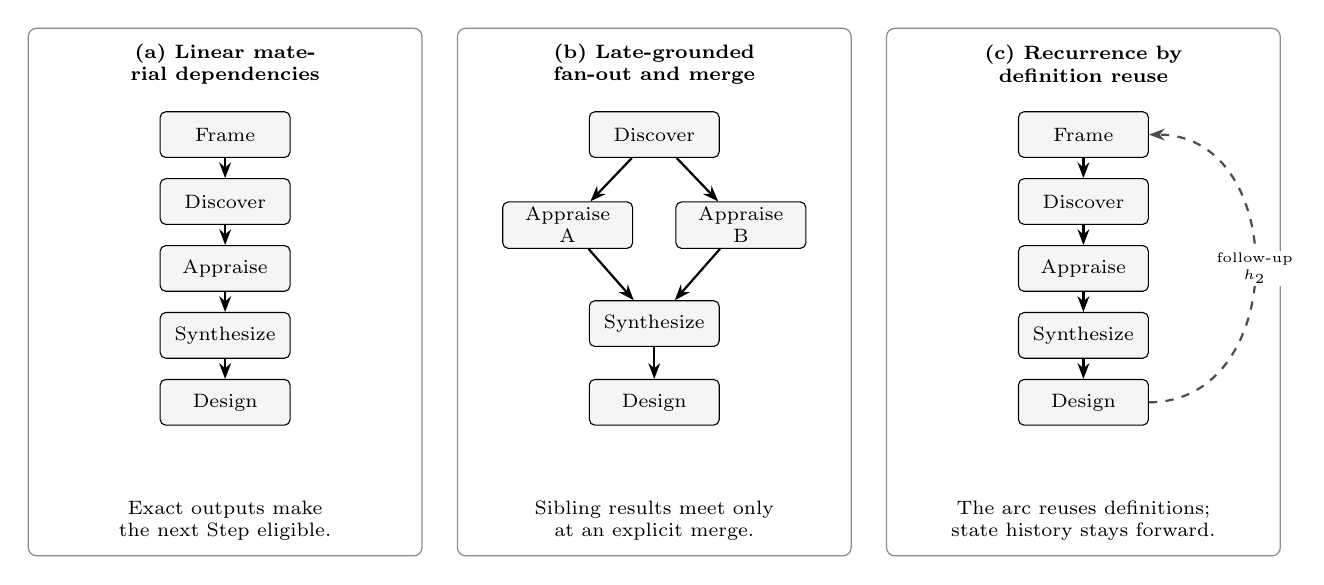
\begin{tikzpicture}[
  box/.style={draw,rounded corners=2pt,minimum width=1.65cm,minimum height=.58cm,
              align=center,font=\scriptsize,fill=black!4,inner sep=2pt},
  edge/.style={-{Stealth[length=2mm]},thick},
  reuse/.style={edge,dashed,draw=black!70},
  label/.style={font=\scriptsize,align=center},
  panel/.style={draw=black!45,rounded corners=3pt,line width=.45pt}
]
  \begin{scope}[shift={(0,0)}]
    \draw[panel] (-2.5,-.7) rectangle (2.5,6.0);
    \node[label,font=\scriptsize\bfseries,text width=4.4cm] at (0,5.55)
      {(a) Linear material dependencies};
    \node[box] (f1) at (0,4.65) {Frame};
    \node[box] (d1) at (0,3.8) {Discover};
    \node[box] (a1) at (0,2.95) {Appraise};
    \node[box] (y1) at (0,2.1) {Synthesize};
    \node[box] (z1) at (0,1.25) {Design};
    \draw[edge] (f1) -- (d1);
    \draw[edge] (d1) -- (a1);
    \draw[edge] (a1) -- (y1);
    \draw[edge] (y1) -- (z1);
    \node[label,text width=4.2cm] at (0,-.25)
      {Exact outputs make the next Step eligible.};
  \end{scope}

  \begin{scope}[xshift=5.45cm]
    \draw[panel] (-2.5,-.7) rectangle (2.5,6.0);
    \node[label,font=\scriptsize\bfseries,text width=4.4cm] at (0,5.55)
      {(b) Late-grounded fan-out and merge};
    \node[box] (d2) at (0,4.65) {Discover};
    \node[box] (a2) at (-1.1,3.5) {Appraise\\A};
    \node[box] (b2) at (1.1,3.5) {Appraise\\B};
    \node[box] (s2) at (0,2.25) {Synthesize};
    \node[box] (z2) at (0,1.25) {Design};
    \draw[edge] (d2) -- (a2);
    \draw[edge] (d2) -- (b2);
    \draw[edge] (a2) -- (s2);
    \draw[edge] (b2) -- (s2);
    \draw[edge] (s2) -- (z2);
    \node[label,text width=4.2cm] at (0,-.25)
      {Sibling results meet only at an explicit merge.};
  \end{scope}

  \begin{scope}[xshift=10.9cm]
    \draw[panel] (-2.5,-.7) rectangle (2.5,6.0);
    \node[label,font=\scriptsize\bfseries,text width=4.4cm] at (0,5.55)
      {(c) Recurrence by definition reuse};
    \node[box] (f3) at (0,4.65) {Frame};
    \node[box] (d3) at (0,3.8) {Discover};
    \node[box] (a3) at (0,2.95) {Appraise};
    \node[box] (y3) at (0,2.1) {Synthesize};
    \node[box] (z3) at (0,1.25) {Design};
    \draw[edge] (f3) -- (d3);
    \draw[edge] (d3) -- (a3);
    \draw[edge] (a3) -- (y3);
    \draw[edge] (y3) -- (z3);
    \draw[reuse]
      (z3.east) to[out=0,in=0,looseness=1.35]
      node[midway,font=\tiny,align=center,fill=white,inner sep=1pt]
        {follow-up\\$h_2$}
      (f3.east);
    \node[label,text width=4.2cm] at (0,-.25)
      {The arc reuses definitions; state history stays forward.};
  \end{scope}
\end{tikzpicture}
\caption{Three structural views of the running research-to-design Playbook.
Panel (a) shows the linear dependency chain created by exact outputs. Panel (b)
shows Discover late-grounding independent Appraise executions and Synthesize
merging their complete result set. Panel (c) adds a dashed loop arc from Design
to Frame: follow-up $h_2$ makes the same Frame definition applicable to a new
binding. The arc depicts recurrence in the Playbook definition; every accepted
execution still adds a new state along forward-only recorded history.}
\label{fig:evolution}
\end{figure*}

\subsection{A linear first reading}

At its coarsest resolution, the running Playbook forms a material-dependency chain:
Frame produces questions, Discover produces a source map, Appraise produces
evidence, Synthesize interprets the evidence, and Design applies the
interpretation. Ordering is a consequence of material availability. Synthesize
does not follow Appraise because an edge moved a token; Synthesize becomes
groundable because exact appraisal-result occurrences now fulfill its declared
input set. The next subsection refines Appraise and Synthesize into
collection-grounded fan-out and merge.

The linear reading gives two basic requirements. Intermediate writes must not
make downstream Steps applicable, because an agent can revise or abandon them.
Conversely, accepted work must have an exact identity, because a filename such
as \texttt{design.md} may be republished with identical or different bytes
during a later pass. The model therefore distinguishes an artifact
\emph{occurrence}, identified by its creating execution and state, from its
content digest.

\subsection{Dynamic branching and explicit merging}

Discover cannot know the useful fan-out before it inspects the questions and
search space. At accepted completion, Discover freezes a finite
\texttt{appraisal-requests} collection. Each member binds one Appraise
execution, so four members yield four independent executions without four
authored copies of the Step. The scheduler may run these executions
concurrently, subject to a capacity policy that does not change their logical
bindings.

A question-level Synthesize execution requires the successful results that
fulfill its exact subset of appraisal requests. The present model also requires
completion of the entire Discover expansion as a conservative readiness barrier, without
treating unrelated appraisal states as inputs or parents.
At completion, Synthesize selects a duplicate-free set of authorized states
whose result occurrences collectively cover the bound requests. The engine,
not the agent, verifies coverage and records those states as parents.

\subsection{Repetition without cyclic history}

Design emits a finite \texttt{followup-research} collection. A nonempty
collection creates a new exact binding for Frame and therefore another forward
research pass. An explicitly empty collection creates no Frame binding. Once
no other binding is eligible or running, the Playbook is \emph{quiescent}.
Quiescence means that no configured work is currently available; it is not a
proof that the design is correct, a goal has been achieved, or later human work
cannot wake the Playbook.
If every Design execution instead publishes a fresh follow-up member, forward
recurrence can continue without a fixed bound even though the recorded history
remains acyclic.

\section{Execution Model}

\subsection{Immutable task states}

Let $\mathcal{N}$ be exact artifact names, $\mathcal{O}$ immutable artifact
occurrences, and $\mathcal{W}$ material workspace checkpoints. A sealed task
state is
\begin{equation}
s=(\mathit{id}_s,w_s,A_s,C_s,Q_s,\rho_s),
\end{equation}
where $\mathit{id}_s$ is a fresh state identifier and $w_s\in\mathcal{W}$ is a
complete checkpoint. $A_s:\mathcal{N}\rightharpoonup\mathcal{O}$ is a partial
map from artifact names to visible occurrences, so a name may be absent; $C_s$
maps collection names to finite frozen member sets; $Q_s$ is a duplicate-free
set of already sealed parent-state identifiers; and $\rho_s$ records the
producing execution, definition revisions, and bound-input provenance. A state
is immutable after publication. Several states may coexist; lineage does not
mark one state as the active truth.

An occurrence identifies a publication event, not only bytes. Republishing
unchanged bytes can create a new occurrence, while an inherited artifact keeps
its prior occurrence identity. Occurrence identity lets a binding state exactly
which work it consumed without making every descendant appear fresh.

The state history $H=(S,E)$ contains edge $(p,s)$ for every $p\in Q_s$.
Because publication may name only already sealed parents and a new state
receives a fresh identity, $H$ is acyclic by construction. An ordinary
execution has one mechanically fixed parent. A merge-capable execution may
select one authorized parent when that state already covers every bound input;
selecting several distinct authorized parents creates a merge transition when
the inputs live on siblings.

\subsection{Definitions, bindings, and collections}

A Playbook revision $P^r$ is a finite set of validated Step-definition
revisions. A definition $d^r$ contains agent instructions, runtime
configuration, input declarations, readiness conditions, an output contract,
and collection relationships. Validation rejects unresolved references and
incompatible collection keys before any Session starts.

A binding $b$ contains exact ordinary occurrences and collection-member
identities. Three grounding forms are sufficient for the running example:
\begin{enumerate}
  \item an ordinary input resolves an exact named occurrence in one sealed
        state;
  \item \texttt{each}(C) enumerates one candidate grounding for every exact
        member of frozen collection $C$; and
  \item \texttt{complete-set}(R) resolves the exact successful results whose
        immutable fulfillment records cover required member set $R$.
\end{enumerate}
Collection membership is never inferred from filename patterns, directory
scans, or natural-language parsing. The producer explicitly declares a finite
collection during completion; the engine validates and freezes the declaration
inside the successor state.

Accepted publication records each declared fulfillment as an exact relation
from a result occurrence to the request member it fulfills. Failed or rejected
executions record no successful fulfillment. Claims, rather than grounding,
suppress duplicate automatic executions for already claimed exact bindings.

Readiness and input resolution are separate operations. Let $u$ be a readiness
witness set and $b$ the exact input binding. A broad condition may establish
that all Appraise requests from one Discover expansion have some successful
result, while a Synthesize binding contains only the results for one question.
The witness states in $u$ do not become input, merge candidates, or lineage
unless their occurrences also appear in $b$.

Automatic duplicate suppression uses a durable claim identity
\begin{equation}
\kappa=\operatorname{ClaimIdentity}(P^r,d^r,b,\chi),
\end{equation}
where $\chi$ is the still-open policy scope, such as ordinary-parent context or
an ancestry scope. Its canonical storage encoding is an implementation choice.
Claim acquisition and queued-execution creation form one atomic operation. A
claim names logical identity; it is not a proof of successful completion.
Explicit manual reruns receive distinct execution identities. Failure retention
and automatic retry policy remain separate decisions rather than hidden parts
of the binding.

\subsection{Executions and Sessions}

A Step execution
\begin{equation}
e=(P^r,d^r,b,A_e,K_e,o_e,W_e,\langle q_1,\ldots,q_k\rangle)
\end{equation}
binds one definition revision to one exact input, a frozen authorized candidate
set $A_e$, required coverage $K_e$, a mechanically fixed ordinary parent
$o_e$ when applicable, an isolated workspace $W_e$, and an ordered sequence of
harness Sessions. At most one Session is write-capable at a time. A continuation
Session receives the same definition, binding, and unpublished workspace; it
does not acquire another claim or create an intermediate state.

Process lifetime is therefore not the semantic boundary. A Session may exit
without completing the execution, and an execution may continue in another
Session. Conversely, a still-live process cannot mutate a state after accepted
completion. The Step execution, rather than its operating-system process, owns
the single publication decision.

\subsection{Validated atomic publication}

An agent requests completion by declaring outputs, collections, and, for a
merge, selected parent identifiers. The engine serializes completion against
continuation, suspends writes, and checks four conditions:
\begin{enumerate}
  \item every required output exists at an allowed path;
  \item every required collection is present, including an explicitly empty
        collection where emptiness is meaningful;
  \item selected parents are duplicate-free members of the candidate set frozen
        in $e$; and
  \item selected parents collectively cover every exact bound input that
        requires cross-state merge.
\end{enumerate}
After validation, the engine checkpoints the complete workspace, assigns
occurrence identities only to declared publications, freezes collections and
fulfillment relationships, constructs the state manifest, and atomically makes
the state and successful execution visible. A rejected completion publishes
nothing and leaves the execution continuable. Explicit failure closes the
execution without a successor and records failure outside the successful state
DAG.

The publication rules give the central visibility invariant:
\begin{equation}
\begin{aligned}
\operatorname{accepted}(e)
  &\Longrightarrow |\operatorname{Successors}(e)|=1,\\
\neg\operatorname{accepted}(e)
  &\Longrightarrow |\operatorname{Successors}(e)|=0.
\end{aligned}
\end{equation}
No downstream evaluation observes a partially checkpointed state or a
successful provenance record without its corresponding state.

\subsection{Reactive evaluation}

Algorithm~\ref{alg:evaluate} gives the event-driven reference behavior.
Grounding and readiness inspect a consistent snapshot of sealed history.
Exact input resolution either waits or returns $(b,A,K,o)$; the atomic
claim-and-create operation freezes those values in the execution record.
Claiming occurs before capacity-limited dispatch, so two evaluator passes cannot
create duplicate automatic executions for the same identity. A scheduler
chooses when queued work starts but cannot change what the binding means.

\begin{algorithm}[tb]
\caption{Reactive grounding, claiming, and publication}
\label{alg:evaluate}
\begin{algorithmic}[1]
\REQUIRE Playbook revision $P^r$, sealed history $H$
\STATE evaluate once when $P^r$ is attached
\LOOP
  \STATE $I \leftarrow \operatorname{Snapshot}(H)$
  \FORALL{$d^r\in P^r$}
    \FORALL{$g\in\operatorname{Ground}(d^r,I)$}
      \STATE $r\leftarrow\operatorname{ResolveExactInputs}(d^r,g,I)$
      \IF{$r=(b,A,K,o)$}
        \STATE $(ready,u)\leftarrow\operatorname{Ready}(d^r,g,b,I)$
        \IF{$ready$}
          \STATE $e\leftarrow\operatorname{ClaimAndCreate}(P^r,d^r,r)$
          \IF{$e\neq\mathsf{none}$}
            \STATE enqueue $e$
          \ENDIF
        \ENDIF
      \ENDIF
    \ENDFOR
  \ENDFOR
  \STATE dispatch queued executions within capacity
  \IF{no unclaimed binding is eligible and no work is queued or running}
    \STATE report quiescence; continue awaiting events
  \ENDIF
  \STATE $x\leftarrow\operatorname{AwaitEvent}()$
  \IF{$x=\operatorname{Completion}(e)$}
    \IF{$\operatorname{ValidateAndPublish}(e,x)$}
      \STATE add the sealed successor to $H$
    \ELSE
      \STATE keep $e$ continuable with validation errors
    \ENDIF
  \ENDIF
\ENDLOOP
\end{algorithmic}
\end{algorithm}

The loop in Algorithm~\ref{alg:evaluate} represents persistent attachment, not
busy polling. Implementations reevaluate on state-sealed and explicit manual
events, and otherwise block. A state publication may ground many executions;
capacity limits dispatch but does not defer claim identity to a mutable future
snapshot. Quiescence is reported after a complete evaluation pass finds no
eligible unclaimed grounding and no queued or running execution, regardless of
whether the preceding event published a state.

\section{The Example as a Concrete Trace}

\subsection{Linear publication boundaries}

Let the seed $S_0$ contain one initial research handoff. Frame executes in an
isolated workspace and publishes $S_1$ with a
\texttt{research-questions} occurrence. Discover binds that exact occurrence,
freezes its source decisions, and publishes $S_2$. Until each completion is
accepted, the next Step sees neither a half-written question list nor a
temporary source map.

The linear trace demonstrates why a full state, rather than an artifact bundle
alone, is the unit of publication. An agent may change code, supporting files,
and several handoffs together. A complete checkpoint makes the transition
auditable and preserves the exact material context for later inspection or a
replay attempt, while the artifact map supplies stable logical names.

\subsection{Fan-out, siblings, and coverage}

Here, $r_{iX}$ denotes the appraisal request pairing question $i$ with source
$X$, and $S_{iX}$ is the sibling state publishing the corresponding appraisal.
Suppose Discover freezes appraisal requests
$r_{1A},r_{1B},r_{2B},r_{2C}$. Four Appraise executions share parent $S_2$ but
receive distinct member bindings. Accepted results create siblings
$S_{1A},S_{1B},S_{2B},S_{2C}$ even if their wall-clock completion order differs.
The runtime never treats a later-finishing sibling as a descendant of an
earlier-finishing sibling.

Synthesize for question 1 binds only successful results fulfilling
$\{r_{1A},r_{1B}\}$. The execution's authorized candidates are frozen when the
binding is resolved. At completion, the agent may select the states that
actually supply those results; the engine accepts only a duplicate-free set
whose union covers both requests. Results for question 2 can serve as a global
readiness witness but cannot silently become parents of question 1. The same
rule lets Design merge only the exact question syntheses it uses.

Separating readiness, binding, and lineage prevents three plausible errors.
First, a state that
merely existed when a Session started does not become a parent. Second, a state
used to establish global readiness does not become an input. Third, repeating
one parent identifier does not satisfy a two-result merge. Parentage records
material dependence rather than temporal proximity.

\subsection{Another pass}

After Design publishes $S_D$, a follow-up member $h_2$ names the exact research
question that could materially change the design. The member is a new binding,
so Frame can execute again under the same definition revision. Subsequent
Discover and Appraise executions create new descendants with new occurrence
and collection identities, even if a question or source key reuses the same
human-readable text.

If Design instead freezes \texttt{followup-research} as the empty set, no Frame
execution is grounded. The Playbook becomes quiescent after all other claimed
work closes. A future manual-publication operation could add another handoff
and wake the same Playbook without rewinding or deleting earlier history; its
authority and interface remain open.

\subsection{Semantic obligations exposed by the trace}

The example yields five obligations for a compatible runtime:
\begin{enumerate}
  \item \textbf{Atomic visibility:} each accepted execution publishes one full
        state; rejected or failed work publishes none.
  \item \textbf{Topology independence:} scheduler order changes latency, not
        sibling or parent relationships.
  \item \textbf{Automatic-claim uniqueness:} each automatic claim identity
        $\kappa$ is acquired at most once.
  \item \textbf{Coverage-preserving merge:} selected parents are authorized and
        collectively supply the bound result occurrences.
  \item \textbf{Forward recurrence:} repeating a Step definition creates a new
        descendant; no concrete history edge points backward.
\end{enumerate}
Any runtime claiming compatibility with the model must preserve these
obligations. The obligations concern execution provenance and publication
topology; the semantic quality of an appraisal or design remains outside the
execution specification.

\section{Related Work and Positioning}

Classical planning supplies precise vocabulary for states, action
applicability, and successor transitions \cite{fikes1971strips}. Hierarchical
task network planning supplies authored task decompositions that a planner
refines toward executable networks \cite{erol1994htn}. Reactive Playbooks use
neither goal search nor search over alternative Step schemas or task networks:
the process definition is fixed, while agent-produced data determines how many
fixed Step executions are late-grounded. The model is therefore closer to execution and monitoring of an
authored process than to plan synthesis.

Workflow languages commonly represent splits, joins, choices, and loops as
control-flow patterns \cite{vanderAalst2003workflow}; statecharts likewise make
control state and transitions explicit \cite{harel1987statecharts}. A Playbook
may be rendered with similar shapes, but its source of truth is exact material
dependency and provenance. The definition view may contain a visual cycle,
whereas the execution view contains only newly published DAG nodes. Avoiding a
cursor is not a claim that workflow formalisms are incapable of the example.
Material-state sufficiency is a design choice that makes it possible to reconstruct why
each agent execution occurred.

Temporal planning for actions with duration distinguishes an action's interval
of execution from the points at which its effects change the state
\cite{fox2003pddl21}. A Playbook Step execution draws a narrower analogous
boundary: several sequential harness Sessions may perform work, but accepted
completion exposes one atomic successor. The paper does not adopt the temporal
constraints, time-varying numeric state variables, or formal plan validation of
the Planning Domain Definition Language (PDDL).

Multi-agent frameworks such as AutoGen provide flexible conversation and tool
interaction patterns \cite{wu2024autogen}. A conversational agent can run
inside a Playbook Session; the Playbook model instead governs durable
publication between executions. General provenance models describe entities,
activities, agents, and derivations \cite{moreau2013prov}. Playbook provenance
specializes that vocabulary with exact input bindings, fulfillment
relationships, automatic claim identity, and coverage-checked state parents.

\section{Limitations and Open Decisions}

This paper specifies execution semantics and illustrates their consequences
with a constructed trace. The example demonstrates that the model represents
this research-to-design pattern; it does not establish a general expressiveness
result, scalability, liveness under failure, agent-output quality,
implementation correctness, or operational security. Claims about those
properties require separate implementation and evaluation work.

Several mechanisms remain policy rather than semantics. A production
specification must settle claim scope across sibling ancestry, retention and
retry after failure, deterministic handling of multiple valid fulfillments,
empty complete-set behavior, merge workspace conflicts, scheduler fairness,
and the representation of manual state creation. Durable publication also
requires a concrete transaction and recovery protocol that prevents a
checkpoint, manifest, claim, and database record from disagreeing after a
crash. External side effects cannot be rolled back merely because filesystem
publication fails.

The model currently assumes one authority creates automatic claims for a task.
Multiple evaluators would require fencing or a shared transactional store.
An isolated workspace is a Playbook visibility boundary, not a security
sandbox; network, subprocess, and external-tool confinement remain outside the
present semantics.
Human interaction is allowed inside a Session and through explicit manual
continuations, yet the paper does not define approval policies or how a human
selects a historical state in the interface.

Finally, the schematic notation in
Appendix~\ref{app:playbook-definition} is not a frozen serialization format.
The semantic distinctions are the intended contract: finite explicit
collections, exact bindings, atomic claims, isolated executions, validated
completion, and coverage-preserving lineage. Locking a portable syntax before
the recovery and authority decisions would turn unresolved policy into
accidental compatibility requirements.

\section{Conclusion}

Reactive Playbooks model long-running agent work as provenance-bound
transitions over immutable material states. One research-to-design definition
consequently expresses linear handoffs, runtime fan-out, concurrent siblings,
coverage-preserving merge, and later refinement without a control cursor or
cyclic history. The reference algorithm makes the governing obligations
explicit: exact grounding, atomic claiming, isolated execution, validated
single-state publication, and fail-closed parent coverage. Recovery, authority,
resource, retry, and serialization policies remain open, but implementations
can resolve those policies against the stable semantic boundary defined here.

{\small
\bibliography{references}
}

\clearpage
\appendix
\section{Schematic Playbook Definition}
\label{app:playbook-definition}

Listing~\ref{lst:playbook} records a compact definition of the running example.
The notation names the semantic relationships used in the paper without
freezing a portable serialization format. Agent instructions, harness
selection, resource policy, and output paths remain part of a complete Step
definition even where the schematic elides them.

\begin{listing}[H]
\begin{lstlisting}
playbook: research-to-design
collections:
  appraisal-requests: key(question, source)
  appraisal-results: fulfills(appraisal-requests)
  question-synthesis-requests: key(question)
  question-syntheses: fulfills(question-synthesis-requests)
  followup-research: key(handoff)
  framed-questions: fulfills(followup-research)
  design-requests: key(design)

steps:
  frame:
    input: each(followup-research)
    output: framed-questions
  discover:
    input: each(framed-questions)
    emit: [appraisal-requests,
           question-synthesis-requests,
           design-requests]
  appraise:
    input: each(appraisal-requests)
    output: appraisal-results
  synthesize:
    input: each(question-synthesis-requests)
    complete-set: required-appraisals(input)
    when: all-appraisals-from-expansion-fulfilled
    output: question-syntheses
  design:
    input: each(design-requests)
    complete-set: required-syntheses(input)
    output: [design.md, followup-research]
\end{lstlisting}
\caption{Schematic research-to-design Playbook. An initial agenda is represented
as the first member of \texttt{followup-research}; later Design executions may
emit another member or an explicitly empty collection.}
\label{lst:playbook}
\end{listing}

\end{document}
